\chapter{空间生长模型}

微观增长动态如何塑造区域增长的宏观趋势的固有性质引起了经济学家,城市研究,流行病传播和统计物理学研究的极大兴趣。这种复杂系统的空间异质性和自组织使其能够产生聚集效应\cite{Keuschnigg13759}。城市作为人类栖息地的密集结构,在工业和金融等领域发挥着微妙的作用,同时为公民提供有效的生活方式。城市的这种优势吸引人们进入城市地区,这加速了城市问题的发展,例如道路网络发展,城市扩张以及它们之间的共同点。除了个人层面的群体动态之外,维度空间上的社区也不同于优先依恋。例如,在城市内部,个人倾向于靠近,形成现代城市,而他们可以很好地适应某些等级结构,但在空间上相隔很远的距离。这些事实表明复杂系统的空间性质解释了观察水平之间的矛盾。虽然这种复杂性带来了系统能力的大量信息和机会,但考虑到共同增长动态的多维约束,预测社区之间的趋势和相互作用一直是困难的。

在错综复杂的城市现象中,空间统计学家们抽象出了以标度律、城市分形为代表的一些理解角度,它们可以解释不同尺度上都成立的一些普适规律。另一方面,这些城市规律可以用随机过程的方法得到复现,这些方法也在一定程度上克服了城市发展难以通过实验验证的困境。此类数理模型的大量研究使得我们有理由相信,这些城市规律可以由更微观的机制来生成,而且这些方法对于未来的预测都是有意义的。本章将综述不同的城市现象对应的统计物理模型,并给出其中重要的原理阐释。

Temporal profiles of avalanches on networks
一个事件引起一个或多个后续事件时,就会发生雪崩或级联,进而可能导致连锁反应中的其他事件。在许多学科中研究雪崩动力学,最近集中在平均雪崩形状上,即固定持续时间的雪崩的时间分布。在动力学的关键点,不同持续时间的重新缩放的平均雪崩形状会塌陷到一条通用曲线上。我们应用马尔可夫分支过程理论来推导控制网络级联动力学的平均雪崩形状的方程。临界状态下的方程分析表明,对于某些动力学和网络拓扑组合,会出现非对称平均雪崩形状(在某些实验中观察到)。我们使用模型的数值模拟来给出示例,以进行信息传播,神经动力学和行为采用,并提出简单的实验测试来量化级联系统是否处于临界状态。
Diffusion in networks and the virtue of burstiness
疾病的蔓延和信息的传播取决于个人的接触。 人们并不总是能够与周围的人互动,并且人们活动的时机决定了人们是否有机会会面和传播细菌,想法等,并最终决定是否会广泛传播或传播。 我们显示,在一个简单的传染或扩散模型中,当活动模式存在异质性时,最大程度的传播发生:有些人长时间处于活动状态,然后长时间不活动,仅偶尔改变其可用性,而 其他人经常在活跃和不活跃之间交替。 这种观察对限制传染性疾病以及促进信息传播具有政策意义。
Effects of Network Structure, Competition and Memory Time
on Social Spreading Phenomena
在线社交媒体极大地影响了我们彼此交流的方式。 但是,人们对什么基本机制驱动在线社交系统中的动态信息流知之甚少。 在这里,我们介绍了一种在线共享行为的生成模型,该模型在分析上易于处理,并且可以重现有关标签使用情况的经验微博数据的多个特征,例如(时间相关的)模因流行度的重尾分布。 所提出的框架构成了社交传播现象的无效模型,与纯粹的经验研究或基于模拟的模型相比,该模型清楚地区分了影响模因流行的两个不同因素的作用:用户的记忆时间和社交网络的连通性结构 。

\section{城市的规模}

人的空间分布表现出从家庭($\sim 0.01$ km)到洲际($\sim 10000$ km)的各种尺度的聚类。通过对经验数据的研究,科学家发现了针对城市规模分布的简单幂律规律(称为齐普夫定律)以及人口密度波动是规模的函数。即\[n(N) \propto N^{−2}.\] 这个函数形式的意义在于,规模越大的城市频率越小,并且随城市的位次是一个幂指数为$-2$的幂律衰减形式。在这里,城市的规模主要指的是人口规模。那么各个城市人口的变化规律

使用随机场理论和统计物理学的技术,我们证明这些幂定律从根本上来说是人类无标度空间集群的结果,也是人类居住在二维表面上的事实。从这个意义上说,两个空间尺度上尺度不变的对称性与城市社会学密切相关。我们通过经验地测量人口密度波动的功率谱来检验我们的理论,并表明对数斜率$\alpha= 2.04\pm0.09$,与我们的理论预测$\alpha= 2$非常吻合。该模型通过导入随机场的数学形式主义。

\subsection{基于偶发过程的城市局部交互标度律模型}

Manrubia, Susanna C.团队在1998年的两篇工作\cite{PhysRevE.58.295, PhysRevLett.79.523}继承了Zeldovich在随机网络的工作,并引领了这个机制在城市科学的相关研究。在人口系统中,地理相关性通常被称为相关场,作为局部人口迁移的动力学机制解释。在总人口为确定值的二维方形格网区域内,记录每一个时刻$t$的每个格点$x$上的人口为$n(x,t)$. 则下一个时刻的人口分布符合\begin{align}
    n(x,t') = \begin{cases}
        (1-q)n(x,t)/p , \text{概率为 } p\\
        qn(x,t)/(1-p) , \text{概率为 } p
    \end{cases}
\end{align}这种机制保证了总人口的恒定,同时增加人口分布的矩$\mu_k(t) = \sum_k n(x,t)^k$. 它的实际意义是不断增加的空间异质性。由于总人口的恒定,该模型可以解释为一个人口迁移模型,即人口不断从乡村区域迁移到城市,迁移到不同城市的速率正比于城市的规模。为了使这个机制得以实现,我们还需要假设对于每一个位置,迁出的人口是该处人口数的一个固定比例$\alpha$。
\begin{figure}[h]
    \centering
    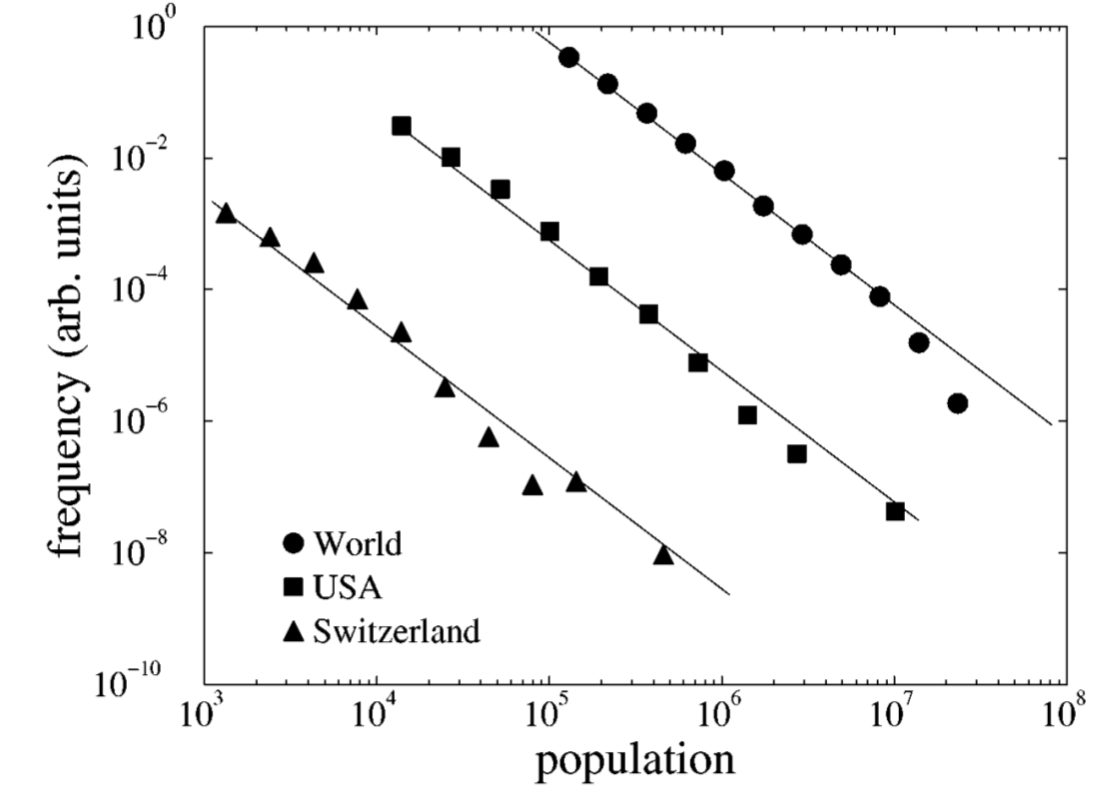
\includegraphics[width = 0.3\linewidth]{pictures/roiiudreal.png}
    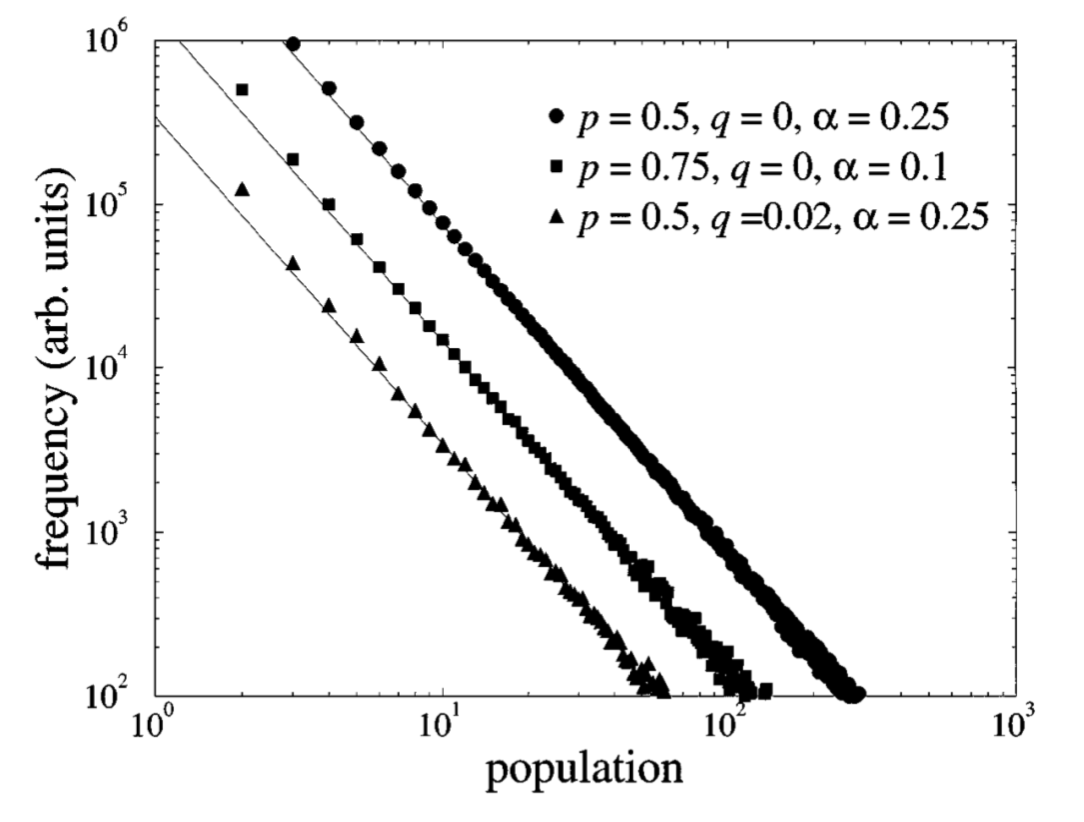
\includegraphics[width = 0.3\linewidth]{pictures/roiiud.png}
    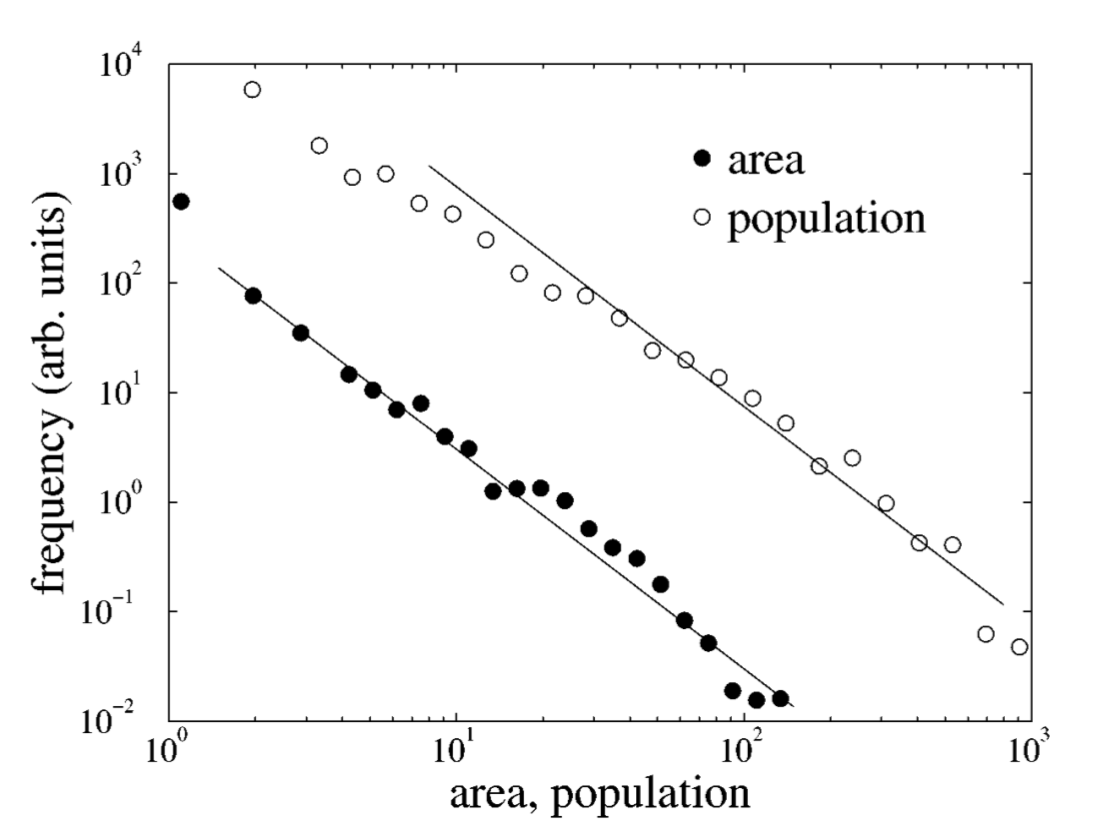
\includegraphics[width = 0.3\linewidth]{pictures/roiiudarea.png}
    \caption{左图:全球2700个最大城市,美国的2400个最大城市和瑞士的1300个最大的自治市的人口分布\cite{PhysRevLett.79.523}. 图中斜率为$-2$ 右图是该文中对于不同的参数的三组模拟结果。我们发现,该模型下不同参数导出的城市人口分布都服从一个参数为$2$的幂律分布。}
\end{figure}该模型可以导出的另一个结果是城市面积的频率。通过假设人口密度高于总人口密度的区域为城市区域,连通的城市区域可以进行面积的统计。城市人口的聚集效应导致城市面积趋近于稳定大小。边际区域上面得到的补充人口与扩散人口数维持动态平衡。结果如图三所示。

基于此类模型,笔者总结了较为一般的模型规律。即反应-扩散模型(reaction-diffusion models)导出空间异质性的基本原理。



% 人类移动性的模式
在此我们额外总结一下人类移动性的模式。通常我们会认为人类的行动是一个连续时间的随机游走(continuous time random walk,即CTRW),与此相关的是数学模型是扩散过程(diffusion limit models)。扩散过程的一个问题是难以解释人类移动的厚尾情形,即现代社会中跨城市尺度的移动。基于此,Mandelbrot提出了列维飞行的概念\cite{doi:10.1142/S0218127408021877}来解释人类移动性的厚尾分布。这两种方式有一个共同的优点,即可以通过随机微分方程的方式得到很多有趣的结论。这两类问题的常用工具Fokker–Planck方程在物理中的意义是粒子在势能场中受到随机力后,随时间演化的位置或是速度的分布函数。这对于我们探究人类移动性对于偶发事件的反应也是有很大帮助的。Chaoming Song于2010年提出的一种双机制模型\cite{song2010modelling}是笔者看到的解释力最强的人类移动性模型。

近年来,相关研究仍在继续。统计规律在新的数据集上并不成立,使得人们对已有模型的动力学机制产生了怀疑。一些研究\cite{GallottiA}表明,列维飞行无法解释私家车轨迹数据集上体现出的行进时间和速度的行为。

而如今,人类移动的模式仍然不能被完全理解。虽然我们仍然对此不解,但却已经是在更高的层次上不解了。人类移动的扩散效应建模的假设里,人的大小是忽略不计的。在进一步研究中,我认为可以将爱因斯坦关系\cite{doi:10.1002/andp.18551700105}融入移动性建模之中,即考虑社会经济条件对人产生的\emph{粘性}。此时在低雷诺数的极限下,迁移率是阻力系数的倒数。我们即可以根据城市的社会经济条件定义城市吸引力,以统一人类移动性在不同城市间的差异性。其中,随机时间点上的的加速而引起的速度变化。将该机制与行程时间的指数衰减结合起来,会导致出行距离的短尾分布,这可能被误解为带截断的幂律分布。这些结果说明了纯描述性模型的局限性,并提供了移动性的机制解释。

升矩过程


\subsection{随机几何模型}

Mathematics and morphogenesis of cities: A geometrical approach

\subsection{基于距离衰减的长程模型}

根据Jürgen P. Kropp在2013年提出的模型\cite{PhysRevE.87.042114},增长更可能发生在居住空间附近。 该模型涉及一个参数,该参数是确定吸引力随距离衰减的强度的指数。 此外,该模型是迭代运行的,因此现有群集可以(一起)增长,并且可以出现新的群集。 该模型能够再现最大聚类边界的大小分布和分形。 尽管幂律分布取决于施加的指数和迭代,但分形似乎独立于前者,而仅取决于后者。

\section{城市活动的空间分布}

Spatial ecology of territorial populations

从植被到生物膜的许多生态系统都是由争夺养分和物理空间的领土人口组成的。这种空间组织对生物多样性有何影响?为了解决这个问题,我们开发并分析了区域资源竞争的模型。在该模型中,所有物种都在新陈代谢的生物物理约束下获得了权衡;该物种占据非重叠领土,而营养物质则在太空中扩散。我们发现养分扩散时间是生物多样性和人口动态时间尺度的重要控制参数。有趣的是,快速的营养扩散使某些物种的种群波动为零,从而导致物种灭绝。此外,领土竞争会自发地产生多重稳定性和Allee效应(在其中需要最少的人口才能生存),因此小规模的扰动会对生态产生重大影响。权衡的假设允许比营养物质数量更多的物种共存(从而违反了竞争排斥的原则),但总体上生物多样性却受到“寡养”物种的控制。重要的是,与充分混合的模型相比,空间结构使多样性对于代谢权衡不平等具有鲁棒性。我们的结果表明,仅由于空间社区中资源的竞争,领土生态系统就可以显示出高生物多样性和丰富的动态。

\subsection{城市内部的标度律}

\subsection{城市空间分隔的物理背景}

1971年,谢林(Schelling)提出了一种模型,如果有太多相反类型的邻居,他们的家庭就会搬家。在本文中,我们将考虑模型的一个总体种群版本,其中将一个城市划分为N个街区,每个街区都有L座房屋。对于某些ρ<1/2,有ρNL红色族和ρNL蓝色族。如果邻里有对等类型的≤ρcL个家庭,他们会感到幸福,否则,他们会感到不高兴。每个家庭搬到每个空置房屋的速度取决于他们当前所在位置和目的地的幸福感。我们的主要结果是,如果邻域较大,则将存在临界值ρb<​​ρd<ρc,因此对于ρ<ρb,这两种类型会随机地均衡分布。当ρ>ρb时,出现一个新的隔离平衡。对于ρb<ρ<ρd,存在双稳态,但是当ρ超过ρd时,随机状态不再稳定。当ρc足够小时,当ρ接近1/2时,随机状态将再次成为平稳分布。如果是这样,则在其之前是双稳态区域。

Hernan A. Makse, Shlomo Havlin 和H. Eugene Stanley在1995年引领了Diffusion-limit aggregation(DLA)模型在城市科学中的研究\cite{MakseModelling}。该模型认为城市的增长方式可能类似于二维粒子聚集体的增长,也有几篇工作\cite{doi:10.1111/j.1538-4632.1991.tb00245.x, BENGUIGUI199513}使用聚类统计物理学的思想对城市增长进行建模。DLA模型预测应该只存在一个大的分形城市,并且可以不使用传入的“发展单位”(例如,代表人员,资金或资源),因此集群的几乎所有增长都发生在城市边缘的尖端。该工作改进了DLA模型。其中与发展单位相关而不是随机添加到集群中的模型,能够更好地再现观察到的城市形态和城市中子集群(“城镇”)的区域分布系统,也可以描述城市增长动态。我们的物理模型与存在密度梯度时的相关渗滤模型相对应,其动机是由于城市地区的发展吸引了进一步的发展。该模型提供了预测城市形态的全局属性(例如缩放行为)的可能性。

\section{城市交通系统的性质}

弹性的概念在自然和工程系统中都有很广泛的应用。它表示了系统从不同的干扰中适应和恢复的能力。尽管弹性是一个在交通系统中管理风险和理解其是如何崩溃的重要概念,但是这个概念在交通系统中的定义和它的统计性质还是缺失的。

本文基于交通堵塞的时空组团,定义了城市中交通弹性的概念。并发现,在2维城市路网和1维高速公路中,弹性的概率分布是无标度的,并且有着相同的标度指数。交通弹性也揭示了时空堵塞组团和恢复时间的关系。这种关系是与微观机制独立的。我们的结果表明,全局的交通弹性可以提供一个更好的设计复杂工程系统的理解。

交通堵塞是城市健康的顽疾。但正如生态系统有康复的能力,在几种情况下,交通也可以逐渐从混乱中恢复。为了描述这种恢复,我们定义了弹性度量,作为描述时空堵塞集团的标准(它也可以被用于其他网络系统)。基于大尺度的GPS数据机,我们从恢复行为中揭示了三个scaling laws,这些law对于任何congestion scale都是通用的。他们在微观尺度上是独立的,包括交通需求的波动与相关的管理机制。我们的弹性scaling结果可以更好地刻画/提高城市交通对于不同类型堵塞的的适应性。
Synchronized flow in oversaturated city traffic
基于具有随机三相交通流模型的数值模拟,我们揭示了过饱和城市交通中的移动队列(移动拥堵)在交通信号上游一定距离处溶解,同时转换为同步流。 已发现,与高速公路交通一样[Kerner,Phys。 Rev. E 85,036110(2012)],这种交通拥堵的吸收作用可以通过强有力的驾驶员速度适应性来解释:车辆之间的时间间隔(空隙)在行进队列(行进拥堵)的上游增加,导致 移动队列解散。 事实证明,在给定的交通信号参数下,速度适应效果越强,信号位置与道路位置之间的平均距离越短,移动队列在该位置处完全溶解,过饱和的交通仅由同步流组成。 将本简报中的城市交通同步流与公路交通同步流进行了比较。

有研究显示,城市交通系统的异质性是由不同城市景观的异质性导致的\cite{}


\section{跨尺度模型}

这个部分里,我们主要叙述与尤尔西蒙模型相关的生长机制。尤尔模型最早见于对种群数量分布的解释\cite{yule1925ii}。

空间依附效应是尤尔模型可以解决人口分布问题的一个出路\cite{Willis}

城市规模研究发现\cite{Keuschnigg13759},集聚效应(大城市的产出高于预期)遵循跨行业数据中鲁棒的“超线性”关系。 但是我们还希望这种模式可以预测的更多的领域,涉及各个城市在许多时间点的动态标度律,我们还期望随着城市人口的增长,各个城市之间出现平行的超线性增长。此预测尚未经过严格测试。 我使用地理编码的微数据估算了1990-2012年瑞典73个劳动力市场区域中城市规模对人均工资的影响。 数据支持所有瑞典城市群的超线性比例尺制度。 但是,与系统层次上的“富人致富”过程相呼应,超线性增长的轨迹仅对于在城市层次结构中占据主导地位的城市而言才非常稳健。

\subsection{生长模型的记忆效应}

城市的发展是历史累积的,是在高度异质性和差异性的环境中不断演化的。而生长模型中,如果将大多数机制建立在无记忆性的指数增长过程中,模型对于复杂历史状况的城市演化规律的解释能力就会有所下降。

生长模型本身的研究过程也在不断引入新的改进机制,从而使得模型仍能预测出较为确定的指标(可解析性,以及更多的考察要素,如Taylor定律\cite{Giometto7755} 。),也能得到更符合实际状况的预测效果。